\documentclass{article}
\usepackage{graphicx}
\usepackage{float}
\usepackage{xcolor}
\usepackage[letterpaper, margin = 1.5cm]{geometry} 
\usepackage[T1]{fontenc} 
\usepackage{amsmath, amsfonts, amssymb, mathtools}
\usepackage{bm}
\usepackage[style=numeric,sorting=none]{biblatex} %Imports biblatex package
\addbibresource{ref.bib} %Import the bibliography file
\usepackage{multicol}
\usepackage[font=footnotesize]{caption}
\setlength{\columnsep}{1.5cm} 


%%%% Document Information %%%%
    \title{The Parker-Sochacki Method vs. Runge-Kutta Methods for Particle Motion in Magnetic Fields
}
    \date{\today}                                   

\begin{document}
% \begin{multicols}{2}
\maketitle

\begin{abstract}
The Parker–Sochacki (PS) method is investigated as an alternative approach for solving the equations of motion for charged particles in magnetic fields. While Runge-Kutta methods, particularly the fixed-step fourth-order (RK4) and the adaptive (RK45), are widely accepted and commonly applied to such problems, the PS method offers a fundamentally different strategy based on power series expansions and auxiliary variables. Through detailed implementations, the PS method is compared against RK4 and RK45 across three physical scenarios: constant, hyperbolic, and dipole magnetic fields. The intent is not to promote one method over another, but to assess the practical viability of the PS method and highlight its comparability to established techniques in terms of accuracy, stability, and computational performance. Results demonstrate that, with proper formulation, the PS method yields consistent and accurate trajectories, making it a useful tool for certain classes of dynamical systems.
\end{abstract}

\section{Introduction}
The study of Ordinary Differential Equations (ODE) and methods for approximation are commonly centered around the use and application of Runge-Kutta methods which iteratively approximate a solution using the weighted averages of slopes. While many variations for this methods exist, the fourth-order Runge-Kutta approximation is the most popular while adaptive Runge-Kutta methods are often employed when problems undergo abrupt changes that aren’t always well captured by the fixed method approach, applying a smaller step size when needed \cite{numericalmethods}.\\

In contrast, the Parker-Sochacki (PS) is a numerical method that  builds upon the classical Picard iteration technique by leveraging power series expansions and successive approximations to solve differential equations more efficiently. In the traditional Picard approach, an ODE with known initial values is solved iteratively, each iteration involves approximating the equation as a power series and progressively refining the solution. When the function involved satisfies appropriate conditions, this process converges to the exact solution. While the Picard method is theoretically powerful and offers high-order accuracy, its practical use has historically been limited due to the algebraic complexity of expanding subsequent expressions. The PS method overcomes this by reformulating the problem into a computationally manageable form by introducing auxiliary variables when necessary to further reduce the complexity of the equation. It systematically determines the coefficients of the power series representing the solution, making the approach practical for a broader range of problems \cite{parker}\cite{wolf}\cite{rudmin}.  \\

This paper investigates the potential of the PS method by examining three applications: the motion of a charged particle in a constant magnetic field, in a hyperbolic magnetic field, and in a dipole field. The detailed mathematical formulation for determining coefficients is provided and each applications is compared to both a fixed-step fourth-order Runge-Kutta (RK4) method and the adaptive-step Runge-Kutta (RK45) method in python and analyzing trajectories and kinetic energy drift which should ideally remain constant. \\

First, to illustrate the power series methods and the concept of an auxiliary variable consider the following example
    \begin{equation}
        \frac{dy}{dx}=y\quad\quad y_0=1
    \end{equation}
To apply either the Picard or PS method, express $y$ as a power series
    \begin{gather}
            y=\sum_{j=0}^\infty y_jx^j=y_0+\sum_{j=1}^\infty y_{j}x^{j}\label{eq:1.1} \\    
            \frac{dy}{dx}=\sum_{i=0}^\infty y_jjx^{j-1}
    \end{gather}
Which can now be substituted into the original ODE:
    \begin{gather}
            \sum_{j=0}^\infty y_iix^{i-1}=\sum_{j=0}^\infty y_jx^j\\
            \sum_{j=-1}^\infty y_{j+1}(j+1)x^{j}=\sum_{j=0}^\infty y_jx^j\\
            \sum_{j=0}^\infty y_{j+1}(j+1)x^{j}=\sum_{j=0}^\infty y_jx^j\\
            y_{j+1}(j+1)x^{j}=y_jx^j\\
            y_{j+1}=\frac{y_j}{(j+1)} \label{eq:1.2} 
    \end{gather}
Equation \ref{eq:1.2} can now be used to calculate the coefficients for Equation \ref{eq:1.1}. Computing the first few coefficients yields
    \begin{equation}
        y_1=1\quad,\quad y_2=\frac{1}{2}\quad,\quad y_3=\frac{1}{6}
    \end{equation}
which gives
    \begin{equation}
        y=1+x+\frac{x^2}{2!}+\frac{x^3}{3!}+\dots
    \end{equation}
resulting in the exact solution
    \begin{equation}
        y=e^x
    \end{equation}
This simple example demonstrates the utilization of a power series representation but has not yet introduced an auxiliary variable. Next, consider the following example
        \begin{equation}\label{eq:1.6} 
        \frac{dy}{dx}=y^2\quad\quad y_0=1
    \end{equation}
where again $y$ can be written as a power series
    \begin{equation}
        y=\sum_{j=0}^\infty y_jx^j=y_0+\sum_{j=1}^\infty y_{j}x^{j}\label{eq:1.3}    
    \end{equation}
Introducing an auxiliary variable $z$ allows for further simplification of the nonlinear term. The introduction of the auxiliary variable is the fundamental difference between the Picard iteration and the Parker-Sochacki method and allows for the use of this approach with non-linear terms.
    \begin{equation}
        z=y^2=\sum_{j=0}^\infty z_jx^j
    \end{equation}
Which is equivalent to
    \begin{equation}\label{EQN:cauchy}
        \begin{split}
            z=&\left(\sum_{j=0}^\infty y_jx^j\right)\left(\sum_{j=0}^\infty y_jx^j\right)\\
            =&\sum_{j=0}^\infty\left(\sum_{k=0}^jy_ky_{j-k}\right)x^j        
        \end{split}
    \end{equation}
therefore
    \begin{equation}
        z_j=\sum_{k=0}^jy_ky_{j-k}
    \end{equation}
Since  
    \begin{equation}
        \frac{dy}{dx}=\sum_{j=0}^\infty (j+1)y_{j+1}x^j
    \end{equation}
this is set equal to Equation \ref{EQN:cauchy} giving
    \begin{gather}
        \sum_{j=0}^\infty (j+1)y_{j+1}x^j=\sum_{j=0}^\infty\left(\sum_{k=0}^jy_ky_{j-k}\right)x^j\\
        y_{j+1}=\frac{1}{(j+1)}\left(\sum_{k=0}^jy_ky_{j-k}\right)\label{eq:1.5}
    \end{gather}
Equation \ref{eq:1.5} now provides the necessary coefficients to compute the solution. Calculating the first few coefficients gives
    \begin{equation}
        \begin{split}
            y_1=y_0y_0=1\\
            y_2=\frac{1}{2}\left(y_0y_1+y_1y_0\right)=1\\
            y_3=\frac{1}{3}\left(y_0y_2+y_1y_1+y_2y_0 \right)=1
        \end{split}
    \end{equation}
Where each of the coefficients can be computed once and used as needed. Utilizing these coefficients in Equation \ref{eq:1.3} results in
    \begin{equation}
        y=1+x+x^2+x^3+\dots=\frac{1}{1-x}
    \end{equation}
which is the exact solution to Equation \ref{eq:1.6}. These two examples demonstrate how the PS method expands on the principles of the Picard iteration by utilizing auxiliary variables and reducing non-linear equations into coupled ODEs that can be solved using algebraic operations. The multiplication of the two summations in Equation \ref{EQN:cauchy} is what is known as a Cauchy Product and has the following form
    \begin{equation}
        \left(\sum_{i=0}^\infty a_i\right)\left(\sum_{j=0}^\infty b_j\right)=\sum_{k=0}^\infty\sum_{l=0}^ka_lb_{k-l}
    \end{equation}
and will appear in many applications of PS method. \\

The next several sections will examine applications of this method for an arbitrary particle in different magnetic field configurations. The intent was not to optimize each of the integration methods and so while some adjustments are made to tolerances and some comments are provided on computation time, this should be taken as a proof of concept. 
\section{Constant Magnetic Field}
This first application will examine the motion of a charged particle in a constant magnetic field. This serves as a foundational application due to its simple, non-trivial nature, allowing for straightforward analysis of the well-understood physics of cyclotron motion governed by the Lorentz Force Law,  
    \begin{equation} \label{eq:2.4} 
        F=m\frac{d\mathbf{v}}{dt}=q\mathbf{v}\times\mathbf{B}
    \end{equation}
where
    \begin{equation}  \label{eq:2.1}
        \frac{d\mathbf{r}}{dt}=\mathbf{v}
    \end{equation}
Letting $\frac{q}{m}=1$ and defining the initial conditions as 
    \begin{equation}
        \begin{split}
            \mathbf{v}(t=0)=\mathbf{v}_0\\
            \mathbf{r}(t=0)=\mathbf{r}_0\\
        \end{split}
    \end{equation}
where $\mathbf{r}$ and $\mathbf{v}$ are the three-dimensional position and velocity vectors, the power series can now be determined.
\subsection{Determining the Power Series Coefficients}
While expressions derived in detail are limited to the $x$-component coefficients, this method can easily be expanded to encompass all other axes. Begin by expressing velocity and position as a power series expansion,
    \begin{equation}\label{eq:2.2}    
        x=\sum_{i=0}^\infty x_it^i 
    \end{equation}
    \begin{equation}\label{eq:2.3}  
        v_x=\sum_{j=0}^\infty v_{xj}t^j    
    \end{equation}
and inserting these into the $x$-component of Equation \ref{eq:2.1} results in
    \begin{equation}
        \begin{split}
            \frac{d}{dt}\left(\sum_{i=0}^\infty x_it^i\right)=& \sum_{j=0}^\infty v_{xj}t^j\\ 
            \sum_{i=0}^\infty ix_it^{i-1}=&\sum_{j=0}^\infty v_{xj}t^j\\ 
        \end{split}
    \end{equation}
In order to develop useful expressions for the coefficients, $t$'s must be of the same order; therefore, the substitution $i=j+1$ is made   
    \begin{equation}
        \begin{split}
            \sum_{j=-1}^\infty (j+1)x_{j+1}t^{j}=&\sum_{j=0}^\infty v_{xj}t^j\\ 
        \end{split}
    \end{equation}
Note that for the summation on the left-hand side, $j=-1$ will result in 0; therefore, with no loss of generality, the summation index can begin at zero. Thus allowing for an expression for the $x$ coefficients
    \begin{equation}\label{eqn: ith_x_constantb}
        x_{j+1}=\frac{v_{xj}}{j+1}
    \end{equation}
which allows us to express Equation \ref{eq:2.2}, as
    \begin{equation}
        {x=\,x_0 + \sum_{j=0}^\infty\frac{v_{xj}}{j+1} t^{j+1}}\\ 
    \end{equation}
Following a similar procedure for velocity, taking the $x$ component of Equation \ref{eq:2.4} and normalizing with respect to $q/m$ then expressing $v_y$ and $v_z$ as power series 
    \begin{equation}
        \begin{split}
        \frac{dv_x}{dt}=&v_yB_z-v_zB_y\\
        \frac{d}{dt}\left(\sum_{j=0}^\infty v_{xj}t^j\right)=&\sum_{k=0}^\infty (v_{yk}B_z-v_{zk}B_y)t^k\\  
        \sum_{j=0}^\infty jv_{xj}t^{j-1}=&\sum_{k=0}^\infty (v_{yk}B_z-v_{zk}B_y)t^k  
        \end{split}
    \end{equation}
To match $t$ coefficients, let $j=k+1$ 
    \begin{equation}
        \begin{split}  
        \sum_{k=-1}^\infty (k+1)v_{x(k+1)}t^{k}=&\sum_{k=0}^\infty (v_{yk}B_z-v_{zk}B_y)t^k  
        \end{split}
    \end{equation}
Again, noting on the left summation that $k=-1$ results is zero; with no loss to generality, the summations index can begin at $k=0$ and thus allowing for an expression for the $v_x$ coefficients
    \begin{equation}\label{eqn: ith_v_constantB}
        v_{x(k+1)}=\frac{1}{k+1} (v_{yk}B_z-v_{zk}B_y) 
    \end{equation}
which allows us to express Equation \ref{eq:2.3} as
    \begin{equation}
            {v_x=v_{x0}+\sum_{k=0}^\infty\frac{1}{k+1} (v_{yk}B_z-v_{zk}B_y)t^{k+1}}
    \end{equation}
To summarize, and extending this methodology to all three dimensions, the following six equations govern the motion of a particle in a magnetic field utilizing the Parker-Sochacki method.
    \begin{gather}
        x=\,x_0 + \sum_{i=0}^\infty\frac{v_{xi}}{i+1} t^{i+1}\\
        y=\,y_0 + \sum_{i=0}^\infty\frac{v_{yi}}{i+1} t^{i+1}\\
        z=\,z_0 + \sum_{i=0}^\infty\frac{v_{zi}}{i+1} t^{i+1}\\
        v_x=v_{x0}+\sum_{i=0}^\infty\frac{1}{i+1} (v_{yi}B_z-v_{zi}B_y)t^{i+1}\\
        v_y=v_{y0}+\sum_{i=0}^\infty\frac{1}{i+1} (v_{zi}B_x-v_{xi}B_z)t^{i+1}\\
        v_z=v_{z0}+\sum_{i=0}^\infty\frac{1}{i+1} (v_{xi}B_y-v_{yi}B_x)t^{i+1}
    \end{gather}
Each $i^{th}$ term from Equation \ref{eqn: ith_x_constantb} and Equation \ref{eqn: ith_v_constantB}, and the respective equations for the other axes, is computed algebraically from the previous ones without the need for further differentiation. Starting from the initial values, a complete set of data points can be formulated.\\
\subsection{Numerical Comparison}
The constant magnetic field provides a valuable baseline for validating numerical methods before progressing to more complex magnetic field configurations. For ease, $q/m$ remains set to unity and a unit-less convention is utilized with a constant magnetic field in the z-direction and an initial velocity in the $v_y$-direction is applied:
    \begin{equation}
        \begin{tabular}{ l l l }
            x_0=0 & v_{x_0}=0 &B_x=0 \\ 
            y_0=0 & v_{y_0}=1  &B_y=0  \\  
            z_0=0 & v_{z_0}=0& B_z=0.1\\
        \end{tabular}
    \end{equation}
Initially, a comparison of the PS and RK4 method was completed, both at fourth order with a fixed time step of 0.63, which equivalent to one hundred steps based on the gyro period of the particle,
    \begin{equation}
        T=\frac{2\pi m}{|q|B}
    \end{equation}
To minimize errors in calculations, an initial time step should be selected which is much smaller than this period, for this scenario 100 steps proved to be conservative\cite{chen}\cite{bird}. Note that the fourth order comparisons are not a one-to-one comparison as the methods are computing different approximations, this merely served as a starting point.\\

Also included in this analysis is the trajectory of an adaptive step RK45 method utilizing \textit{solve$\_$ivp} in python, which numerically integrates the problem utilizing the RK45 method \cite{scipy}. As see in Figure \ref{fig: usecase1-1, trajectory}, all trajectories match the analytical solution very well with near identical errors in trajectory for the RK4 and PS method but a lower trajectory error for the RK45 method, Figure \ref{fig: usecase1-1, trajectory error}. Early analysis utilized the built-in tolerance levels for \textit{solve$\_$ivp} which are 1e-3 for the relative tolerance and 1e-6 for the absolute tolerance \cite{scipy}; however, energy drift errors were on the order of $10^{-1}$ when used in this application and the tolerances were manually updated to 1e-12 and 1e-14, respectively for this analysis. 
        \begin{figure}[H]
            \centering
            \begin{minipage}[t]{0.48\textwidth}
                \centering
        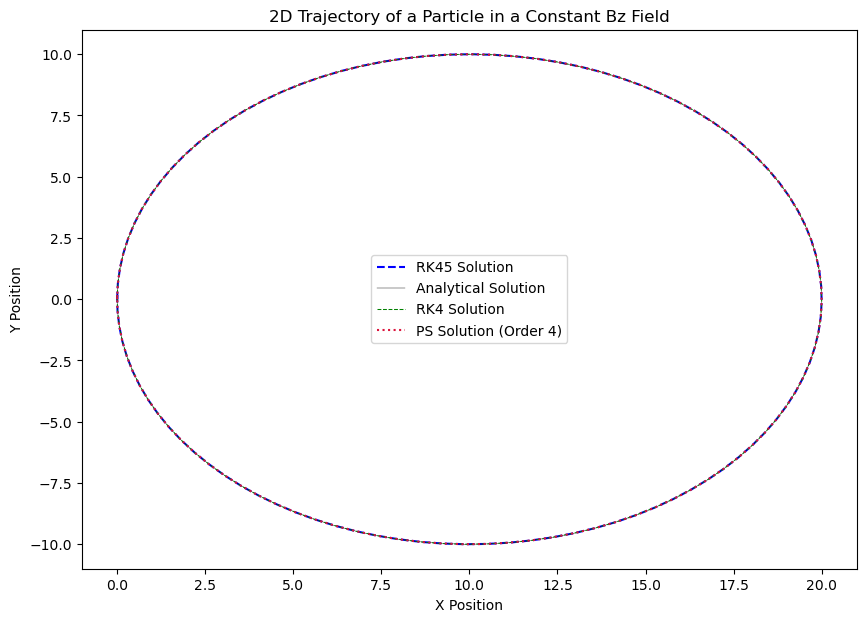
\includegraphics[width=.9\textwidth]{Images/ConstantB/PS_Order4_trajectory_comparison_UseCase1-1.png}
        \caption{2D trajectory of a charged particle in a constant magnetic field along the $z$-axis, computed using the Parker–Sochacki method and two different Runge-Kutta methods (fixed-step fourth order, RK4, and adaptive, RK45) compared to the analytical solution.}
        \label{fig: usecase1-1, trajectory}
            \end{minipage}%
            \hfill
            \begin{minipage}[t]{.48\textwidth}
                \centering
                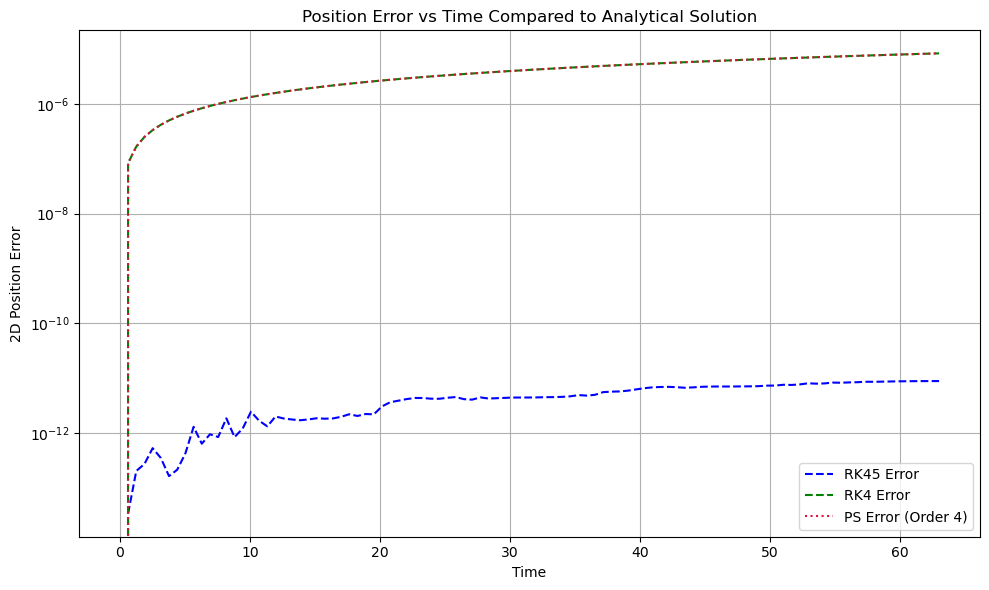
\includegraphics[width=0.9\textwidth]{Images/ConstantB/PS_Order4_trajerror_comparison_UseCase1-1.png}
                \caption{2D trajectory error of a charged particle in a constant magnetic field along the $z$-axis, computed using the Parker–Sochacki method and two different Runge-Kutta methods (fixed-step fourth order, RK4, and adaptive, RK45) compared to the analytical solution.}
                \label{fig: usecase1-1, trajectory error}
            \end{minipage}
        \end{figure}
Additionally, when analyzing at the relative energy error over time, the PS and RK4 methods exhibit near identical error drift, while the RK45 method was lower, Figure \ref{FIG: ConstantB_energyerror_1cycle}.
         \begin{figure}[H]
            \centering
            \captionsetup{width=0.48\textwidth}
            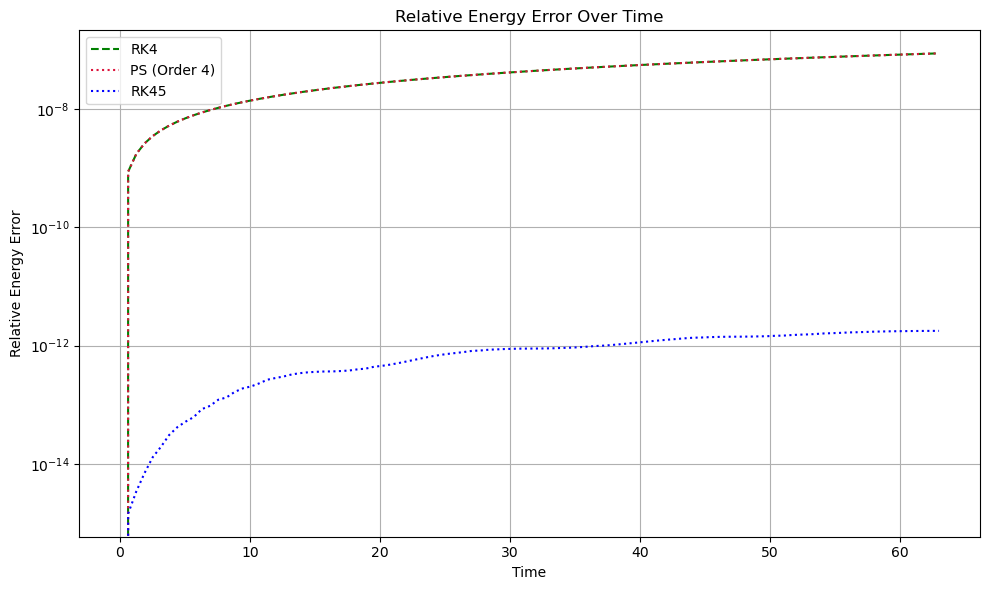
\includegraphics[width=0.4\textwidth]{Images/ConstantB/PS_Order4_energy_comparison_UseCase1-1.png}
            \caption{Energy error of a charged particle in a constant magnetic field along the $z$-axis, computed using the Parker–Sochacki method and fixed-step Runge-Kutta, both to 4$^{\text{th}}$ order.}
            \label{FIG: ConstantB_energyerror_1cycle}
        \end{figure}
           
Next, various PS orders were analyzed over a time scale equivalent to ten orbits, while maintaining a time step of 0.63. Allowing for increased PS orders, reduced both the errors in the trajectory, Figure \ref{FIG:ConstantB_trajerror_stacked}, and the errors in the energy drift, Figure \ref{FIG:ConstantB_engerror_stacked}, by several orders of magnitude, while at times approaching machine error for higher order PS coefficients, with minimal impact to the computation time.
        \begin{figure}[H]
            \centering
            \begin{minipage}[t]{0.48\textwidth}
                \centering
                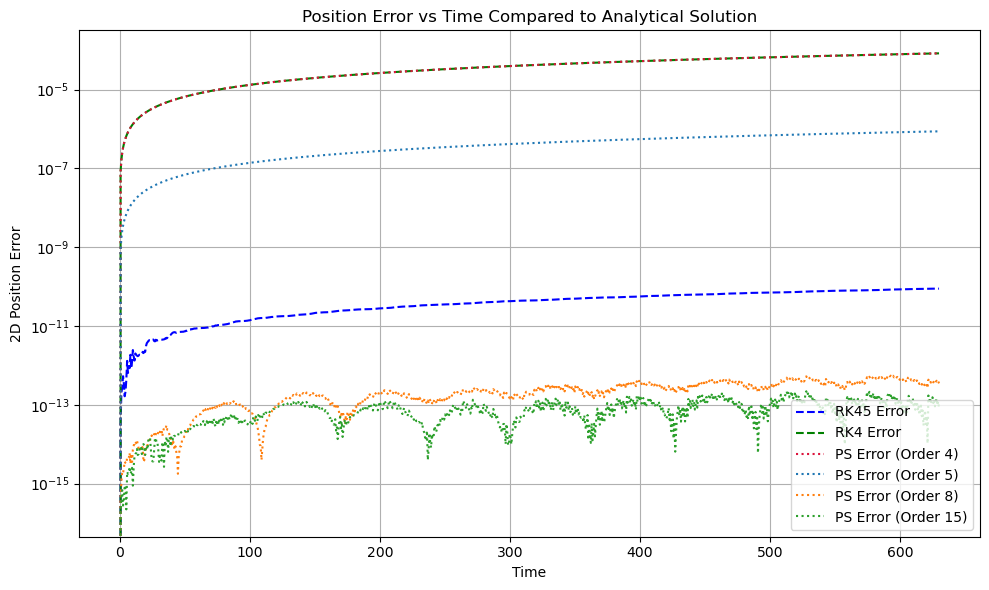
\includegraphics[width=\textwidth]{Images/ConstantB/PS_StackedOrders_trajerror_comparison_UseCase1-1.png}
                \caption{2D trajectory error of a charged particle in a constant magnetic field along the $z$-axis, computed using the Parker–Sochacki method at various orders and both a fixed-step 4th Order and adaptive step Runge-Kutta.}
                \label{FIG:ConstantB_trajerror_stacked}
            \end{minipage}%
            \hfill
            \begin{minipage}[t]{0.48\textwidth}
                \centering
                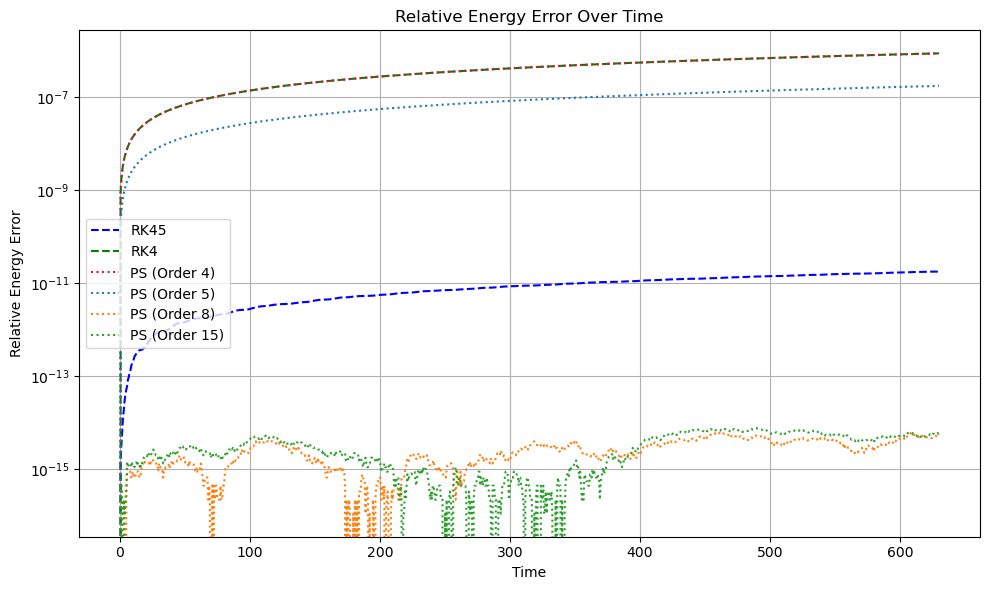
\includegraphics[width=\textwidth]{Images/ConstantB/PS_StackedOrders_energy_comparison_UseCase1-1.png}
                \caption{Energy drift of a charged particle in a constant magnetic field along the $z$-axis, computed using the Parker–Sochacki method at various orders and both a fixed-step 4th Order and adaptive step Runge-Kutta.}
                \label{FIG:ConstantB_engerror_stacked}
            \end{minipage}
        \end{figure}
        
    
This application demonstrate long term stability in the energy drift and more precise calculations due to the higher order terms in the PS method. Even with higher order terms, in this application, the PS method reliably exhibited comparable computation times as the RK4 method. The RK45 method, while consistently the fastest, also exhibited significantly higher error drift over time unless adjustments to the built in tolerances were made allowing for a competitive error drift, which is what was included in the above analysis. Other variations of this analysis, such as reducing the step size down to .05, and examining the helical motion in three dimensions were explored demonstrating similar trends as those summarized above. Lastly, while the RK4 drift error can be decreased further it requires a smaller time step, significantly increasing the computation costs which for longer calculations becomes computationally significant. 

\section{Hyperbolic Magnetic Field}
A hyperbolic magnetic field introduces non-uniformity and non-linearity in a magnetic field environment allowing for the exploration of more practical problems in space physics where sharper changes in the equations can occur over shorter time scales. The field can be representative of the Earth's Magnetotail current sheet, magnetic reconnection, and plasma mirrors [\textcolor{red}{blue textbook reference}]. Unlike a constant magnetic field, the motion of a particle is no longer symmetric and can lead to chaotic behavior where particle trajectories can range from extremely trochoidal to meandering, this behavior is sensative to the combination of position, velocity and magnetic field strength \cite{astrom}. This allows for a more stressing analysis on numerical methods. This application will specifically explore particles that follow the Lorentz Force Law,
    \begin{equation} 
        F=m\frac{d\mathbf{v}}{dt}=q\mathbf{v}\times\mathbf{B}
    \end{equation}
where
    \begin{equation}  
        \frac{d\mathbf{r}}{dt}=\mathbf{v}
    \end{equation}
    \begin{equation}
        \mathbf{B}=\begin{pmatrix}
            0\\0\\\tanh (y)
        \end{pmatrix}
    \end{equation}
For ease, the problem is normalized to $q/m$ and the initial conditions are defined as 
    \begin{equation}
        \begin{split}
            \mathbf{v}(t=0)=\mathbf{v}_0\\
            \mathbf{r}(t=0)=\mathbf{r}_0\\
        \end{split}
    \end{equation}
where $\mathbf{r}$ and $\mathbf{v}$ are the 3 dimensional position and velocity vectors.
\subsection{Determining the Power Series}
Similar to the first application with constant $\mathbf{B}$,
    \begin{equation}    
        x=\sum_{i=0}^\infty x_it^i 
    \end{equation}
    \begin{equation}
        v_x=\sum_{j=0}^\infty v_{xj}t^j    
    \end{equation}
but now an additional term must be introduced for magnetic field which is no longer constant, where an auxiliary variable, $a$, can be introduced
    \begin{gather}\label{equation: Hyper Bz Basic}
        B_z=\sum_{k=0}^\infty B_{z,k}t^k\\
        \frac{dB_z}{dt}=[1-\tanh^2(y)]\frac{dy}{dt}=\underbrace{(1-B_z^2)}_a v_y\\
        \frac{dB_z}{dt}=av_y
    \end{gather}       
therefore,
    \begin{gather}
        \frac{da}{dt}=-2B_z\frac{dB_z}{dt}\\
        a=\sum_{l=0}^\infty a_lt^l
    \end{gather}
Where at $t=0$, the initial conditions are
    \begin{equation}
        \begin{split}
            B_{z0}=\tanh(y)\\
            a_0=1-B_{z0}^2
        \end{split}
    \end{equation}
Examining the auxillary variable, $a$, it can be shown that
    \begin{equation}
        \begin{split}
            a=&\sum_{l=0}^\infty a_lt^l\\
            \frac{da}{dt}=&\sum_{l=0}^\infty la_lt^{l-1}\\
            -2B_z\frac{dB}{dt}=&\sum_{l=0}^\infty la_lt^{l-1}\\
            -2\left(\sum_{m=0}^\infty B_{z,m}t^m\right)\left(\sum_{k=0}^\infty kB_{z,k}t^{k-1}\right)=&\sum_{l=0}^\infty la_lt^{l-1}
            \end{split}
    \end{equation}
when $k=0$ the left side is zero so with no loss to generality the summation index can begin at $k=1$ and let $j=k-1$. Applying similar logic to the right and letting $l-1=i$ gives            
    \begin{equation}
        \begin{split}            
            -2\left(\sum_{m=0}^\infty B_{z,m}t^m\right)\left(\sum_{j=0}^\infty (j+1)B_{z,j+1}t^{j}\right)=&\sum_{i=0}^\infty (i+1)a_{i+1}t^{i}\\
            -2\sum_{i=0}^\infty\sum_{j=0}^i(j+1)B_{z,i-j}B_{z,j+1}t^{i}=&\sum_{i=0}^\infty (i+1)a_{i+1}t^{i}\\
        \end{split}
    \end{equation}
    \begin{equation}\label{eqn: ith a hyper}
        a_{i+1}=-\frac{2}{(i+1)}\sum_{j=0}^i(j+1)B_{z,i-j}B_{z,j+1}
    \end{equation}
 Equation \ref{eqn: ith a hyper} provides the necessary framework to compute the auxiliary coefficients for $a$. Examining $\mathbf{B_z}$, and following a similar mathematical progression, 
    \begin{equation}
        \begin{split}
            \frac{dB_z}{dt}=&\frac{d}{dt}\left(\sum_{k=0}^\infty B_{z,k}t^k\right)\\
            av_y=&\sum_{k=0}^\infty kB_{z,k}t^{k-1}\\
            \left(\sum_{l=0}^\infty a_lt^l\right)\left(\sum_{m=0}^\infty v_{y,m}t^m\right)=&\sum_{k=0}^\infty kB_{z,k}t^{k-1}\\                  
            \sum_{n=0}^\infty \left(\sum_{j=0}^n a_jv_{y,n-j}\right)t^n=&\sum_{k=0}^\infty kB_{z,k}t^{k-1}\\
        \end{split}
    \end{equation}
which reduces to the following
    \begin{equation}\label{equation:Hyper Bz Coefficients}
            B_{z,i+1}=\frac{1}{i+1}\sum_{j=0}^i a_jv_{y,i-j}
    \end{equation}
Equation \ref{equation:Hyper Bz Coefficients} gives the necessary framework to calculate any number of coefficients allowing for a full magnetic field representation of  
    \begin{equation}\label{eqn_ith_B_hyper}
        B_z=B_{z,0}+\sum_{i=0}^\infty \frac{t^{i+1}}{i+1}\sum_{j=0}^i a_jv_{y,i-j}
    \end{equation}

The remaining equations, which were derived in detail in the previous sections, are summarized as follows
    \begin{gather}
        x=\,x_0 + \sum_{i=0}^\infty\frac{v_{xi}}{i+1} t^{i+1}\\
        y=\,y_0 + \sum_{i=0}^\infty\frac{v_{yi}}{i+1} t^{i+1}\\
        z=\,z_0 + \sum_{i=0}^\infty\frac{v_{zi}}{i+1} t^{i+1}\\
        v_x=v_{x0}+\sum_{i=0}^\infty\frac{1}{i+1} (v_{yi}B_{zi})t^{i+1}\\
        v_y=v_{y0}+\sum_{i=0}^\infty\frac{1}{i+1} (-v_{xi}B_{zi})t^{i+1}\\
        v_z=v_{z0}
    \end{gather}
Each $i^{th}$ term from Equation \ref{eqn: ith a hyper} and Equation \ref{equation:Hyper Bz Coefficients}, and the respective equations for the other axes, is computed algebraically from the previous ones without the need for further differentiation and providing a complete set of equations that govern the trajectory of a particle in a hyperbolic magnetic field.

\subsection{Numerical Comparison}
Given the sharp behavior exhibited by a hyperbolic magnetic field, a smaller step size of 0.001 was initially used for the presented analysis and simulations ran for total time of 100. For ease, the problem is normalized to $q/m$ and a unit-less convention is utilized.  Lastly, an $\alpha$ term was introduced to easily scale the magnetic field, while the analysis presented utilized $\alpha=1$, some brief observations on initial observations will be provided at the end of the section on variations of $\alpha$. The remaining initial conditions used were:
    \begin{equation}
        \begin{tabular}{ l l l }
            x_0=0 & v_{x_0}=0 &B_x=0 \\ 
            y_0=.5 & v_{y_0}=.1  &B_y=0  \\  
            z_0=0 & v_{z_0}=.5& B_z=\tanh(\alpha y)\\
        \end{tabular}
    \end{equation}
The PS method was implemented to allow for an adaptive order that would break the loop at a tolerance of 1e-20, which resulted in a PS order of 6. As seen in Figure \ref{FIG:Hyper_Traj_100s}, both RK methods and the PS method exhibit similar trajectories over the simulation and maintain low energy drift, Figure \ref{FIG:Hyper_Error_100s}, both exhibiting the expected trochoidal sort of behavior 

\begin{figure}[H]
    \centering
    \begin{minipage}[t]{0.4\textwidth}
        \centering
        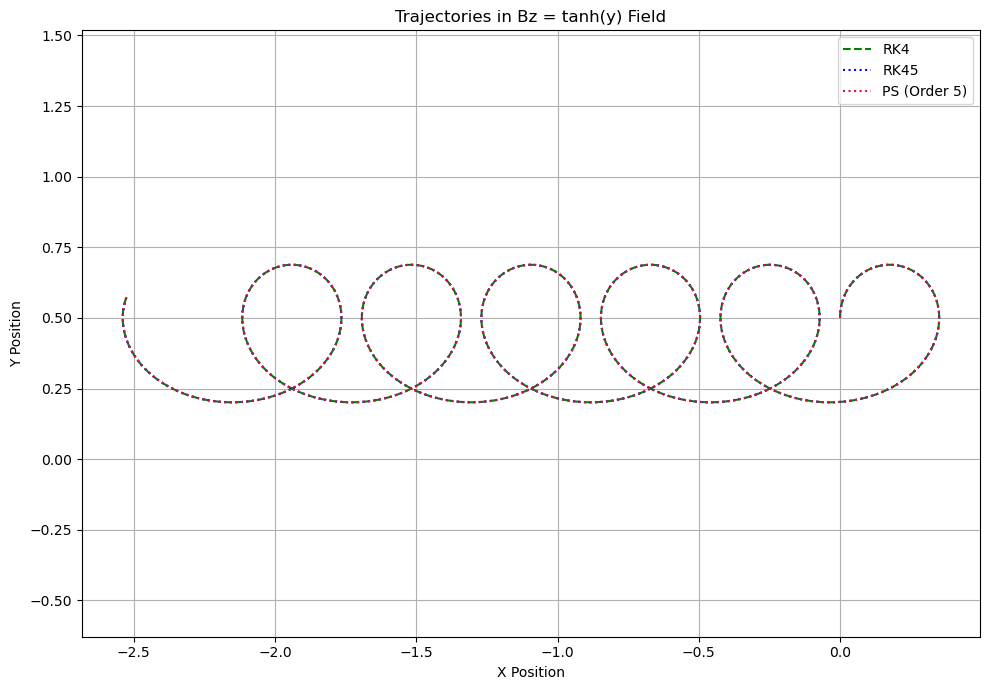
\includegraphics[width=\textwidth]{Images/hyper/Hyper_traj_qm1_alpha1_100s_PS_Order5.png}
        \caption{2D trajectory of a charged particle in a hyperbolic magnetic field computed using the Parker–Sochacki method and two different Runge-Kutta methods (fixed-step fourth order, RK4, and adaptive, RK45).}
        \label{FIG:Hyper_Traj_100s}
    \end{minipage}%
    \hfill
    \begin{minipage}[t]{0.45\textwidth}
        \centering
        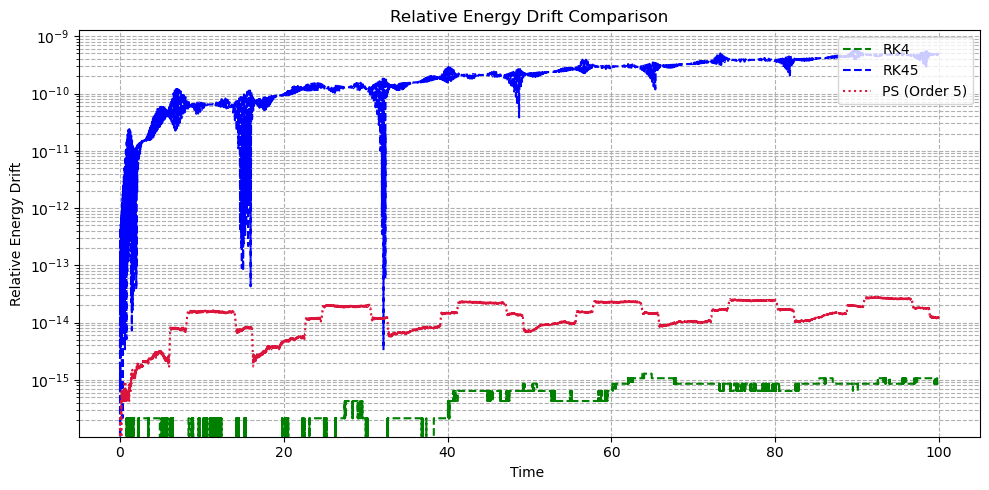
\includegraphics[width=\textwidth]{Images/hyper/Hyper_energydrif_qm1_alpha1_100s_PS_Order5.png}
        \caption{Energy drift of a charged particle in a hyperbolic magnetic field computed using the Parker–Sochacki method and two different Runge-Kutta methods (fixed-st
        ep fourth order, RK4, and adaptive, RK45).}
        \label{FIG:Hyper_Error_100s}
    \end{minipage}
\end{figure}

        
    
For increasing magnetic fields, large $\alpha$, a smaller time step was required to maintain accuracy. In particular, it was observed that smaller time steps were required for the PS method sooner than they were required for the RK4 method as the magnetic field was increased. This is likely due to how each method approximates in sharp regions, one approximating the solution with a higher order polynomial, which can become unstable in the presence of sharp gradients, while the other uses a lower-order approximation that is more stable but less accurate. However, as the PS method only requires addition, subtraction and multiplication, increasing step size for PS method did not have the same computational penalty that RK approximations may face with decreased step size. For example, the following run was conducted for $\alpha=10$  and the following initial parameters.\\


\begin{equation}
        \begin{tabular}{ l l l }
            x_0=0 & v_{x_0}=.1 &B_x=0 \\ 
            y_0=.25 & v_{y_0}=0  &B_y=0  \\  
            z_0=0 & v_{z_0}=0& B_z=\tanh(\alpha y)\\
        \end{tabular}
    \end{equation}
\begin{figure}[H]
    \centering
    \begin{minipage}[t]{0.4\textwidth}
        \centering
        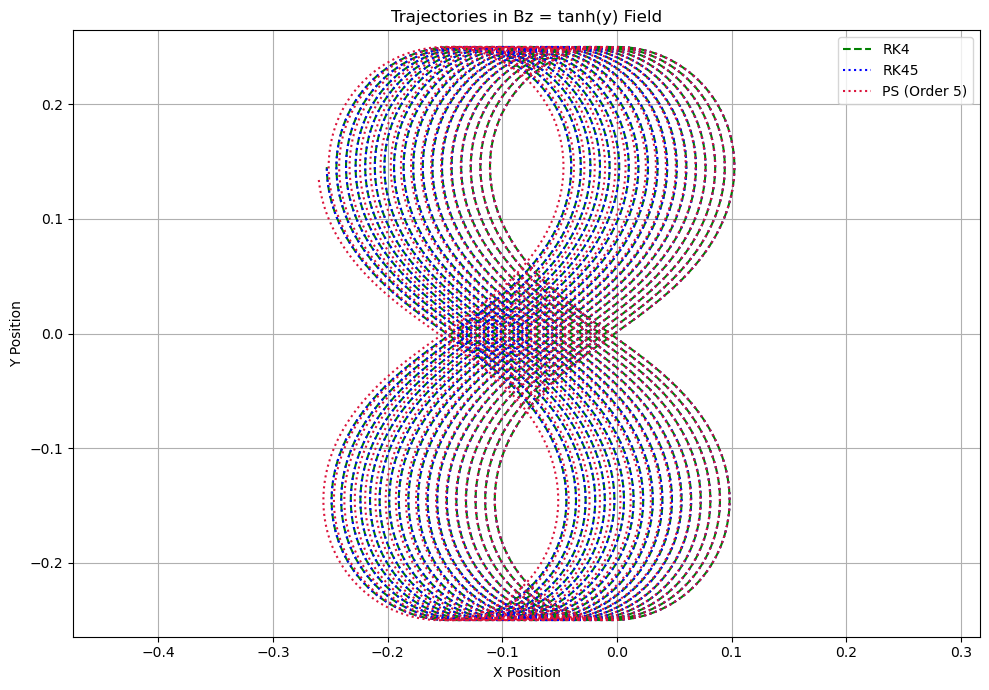
\includegraphics[width=\textwidth]{Images/hyper/Hyper_traj_qm1_alpha10_250s_PS_Order5.png}
        \caption{2D trajectory of a charged particle in a hyperbolic magnetic field computed using the Parker–Sochacki method and two different Runge-Kutta methods (fixed-step fourth order, RK4, and adaptive, RK45).}
        \label{FIG:Hyper_Traj_100s}
    \end{minipage}%
    \hfill
    \begin{minipage}[t]{0.45\textwidth}
        \centering
        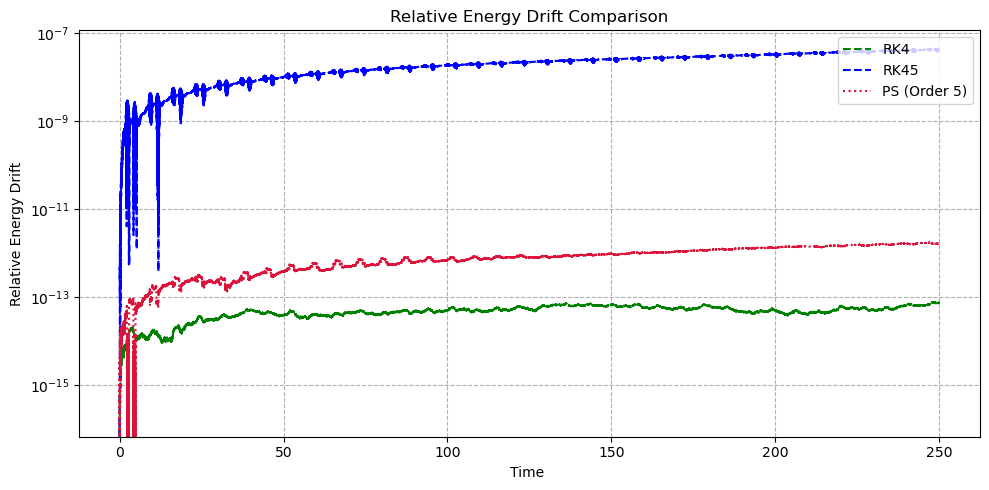
\includegraphics[width=\textwidth]{Images/hyper/Hyper_energydrif_qm1_alpha10_250s_PS_Order5.png}
        \caption{Energy drift of a charged particle in a hyperbolic magnetic field computed using the Parker–Sochacki method and two different Runge-Kutta methods (fixed-step fourth order, RK4, and adaptive, RK45).}
        \label{FIG:Hyper_Error_100s}
    \end{minipage}
\end{figure}

For weaker magnetic field, smaller $\alpha$, all methods performed extremely well by both maintaining energy conservation and minimizing computation costs. The adaptive RK45 remained the fastest, though the internal tolerances had to be adjusted to account and correct for noticeable drift in the trajectory when initially using the default tolerances.   \\


While not quantitatively bound as part of this effort, there appears to be a tradeoff points between the methods depending on both the extremes of the trajectory desired, legnth of run, and other analysis priorities.

\section{Magnetic Dipole}
The final application examines the complex motion of a particle in a dipole field, it provides a robust case study for analyzing the behavior and capabilities of each method. A particle with an initial velocity with both perpendicular and a parallel components, relative to the magnetic field, will experience both a circular motion perpendicular to the magnetic field, as was discussed in the first application, as well as oscillatory motion both along the field line and a drift motion perpendicular to the field line [\textcolor{red}{bluebook reference}].
\begin{equation}   
        F=m\frac{d\mathbf{v}}{dt}=q\mathbf{v}\times\mathbf{B}
    \end{equation}
with 
    \begin{equation} 
        \mathbf{B(r)}=\frac{\mu_0}{4\pi}\cdot\frac{3(\mathbf{m\cdot\hat{r}})\mathbf{\hat{r}}-\mathbf{m}}{r^3}
    \end{equation}
where $\mathbf{m}=m\hat{z}$ so that 
    \begin{equation}
        \mathbf{B(r)}=\frac{\mu_0}{4\pi}\cdot\frac{3m\mathbf{\hat{r}}-\mathbf{m}}{r^3}
    \end{equation}
or explicitly,
    \begin{align}
        B_x=&\frac{\mu_0m}{4\pi}\frac{3xz}{r^5}\\
        B_y=&\frac{\mu_0m}{4\pi}\frac{3yz}{r^5}\\
        B_z=&\frac{\mu_0m}{4\pi}\frac{3z^2-r^2}{r^5}
    \end{align}
\subsection{Determining the Power Series}
Given the following equations
    \begin{align} 
        x=\sum_{i=0}^\infty x_it^i\quad\quad y=\sum_{i=0}^\infty y_it^i\quad\quad z=\sum_{i=0}^\infty z_it^i
    \end{align}
the following auxiliary variables, remembering that each is considered to be an expansion in $t$, can be established    
    \begin{align}
            \beta=xz=\left(\sum_{i=0}^\infty x_it^i\right)\left(\sum_{i=0}^\infty z_it^i\right)=\sum_{i=0}^\infty\left(\sum_{j=0}^i z_jx_{i-j} \right)t^i
      \end{align}
such that 
    \begin{align}
        \beta_i=\sum_{j=0}^i z_jx_{i-j} 
    \end{align}

    \begin{align}
            \gamma=yz=\left(\sum_{i=0}^\infty y_it^i\right)\left(\sum_{i=0}^\infty z_it^i\right)=\sum_{i=0}^\infty\left(\sum_{j=0}^i z_jy_{i-j} \right)t^i
    \end{align}
such that
    \begin{align}
        \gamma_i=\sum_{j=0}^i z_jy_{i-j}
    \end{align}
Noting the $z^2$ will be the only auxiliary variable needed explicitly, $x^2$ and $y^2$ are only needed implicitly for $r$, gives
    \begin{align}
        x^2=\left(\sum_{i=0}^\infty x_it^i\right)^2=\sum_{i=0}^\infty\left(\sum_{j=0}^i x_jx_{i-j} \right)t^i\label{EQN:dipole_x^2}\\
        y^2=\left(\sum_{i=0}^\infty y_it^i\right)^2=\sum_{i=0}^\infty\left(\sum_{j=0}^i y_jy_{i-j} \right)t^i\label{EQN:dipole_y^2}\\
        \epsilon=z^2=\left(\sum_{i=0}^\infty z_it^i\right)^2=\sum_{i=0}^\infty\left(\sum_{j=0}^i z_jz_{i-j} \right)t^i\label{EQN:dipole_z^2}
    \end{align}
such that 
    \begin{align}
        \epsilon_i=\sum_{j=0}^i z_jz_{i-j}
    \end{align}
Equations \ref{EQN:dipole_x^2}, \ref{EQN:dipole_y^2}, and \ref{EQN:dipole_z^2} give
    \begin{equation}
        r^2=\sum_{i=0}^\infty \left(\sum_{j=0}^i x_jx_{i-j}+y_jy_{i-j}+z_jz_{i-j}\right)t^i
    \end{equation}
Finally, the remaining auxiliary variables are established to address $r^{-5}$,
\begin{align}
    a &= r^2 = \sum_{i=0}^\infty a_i t^i \\
    b &= a^{-5/2} = \sum_{i=0}^\infty b_i t^i \\
    c &= \frac{1}{a} = \sum_{i=0}^\infty c_i t^i
\end{align}
where 
    \begin{align}
        a_i=\sum_{j=0}^i x_jx_{i-j}+y_jy_{i-j}+z_jz_{i-j}\label{eqn:afordipole}
    \end{align}
A recursion relationship for $c$ can be developed by noting the following
\begin{equation}
ca=\sum_{i=0}^\infty a_it^i\sum_{j=0}^\infty c_jt^j=\sum_{i=0}^\infty\left(\sum_{j=0}^i a_jc_{i-j} \right)t^i=1\\
\end{equation}
Therefore, $a_0c_0=1$ and all other terms can be summarized as follows 
\begin{align}
\sum_{j=0}^i a_jc_{i-j} =0\quad\text{for } i>0\\
c_ja_0+ \sum_{j=1}^i a_jc_{i-j} =0\quad\text{for }i>0\\
c_i=-\frac{1}{a_0} \sum_{j=1}^i a_jc_{i-j}\quad\text{for } i>0 \label{eqn:cfordipole}
\end{align}

Finally, to build out the recursion relationship for $b$, take the time derivative of the power series, giving

\begin{align}
    \frac{db}{dt} = -\frac{5}{2} \cdot b \cdot c \cdot \frac{da}{dt}
\end{align}

    \begin{equation}
        \begin{split}
        \sum_{i=0}^\infty (i+1)b_{i+1} t^i =& -\frac{5}{2}
        \left( \sum_{i=0}^\infty b_i t^i \right)
        \left( \sum_{j=0}^\infty c_j t^j \right)
        \left( \sum_{k=0}^\infty (k+1) a_{k+1} t^k \right)\\
        =&-\frac{5}{2}
        \left[ \sum_{i=0}^\infty \left(\sum_{j=0}^i b_jc_{i-j}\right)t^i \right]
        \left( \sum_{k=0}^\infty (k+1) a_{k+1} t^k \right)\\
        =&-\frac{5}{2}
         \sum_{i=0}^\infty \left(\sum_{k=0}^i(k+1)a_{k+1}\sum_{j=0}^{i-k}b_jc_{i-k-j} \right)t^i 
        \\
        \end{split}
    \end{equation}
and comparing the coefficients of $t^i$ on both sides gives the recurrence relation 
    \begin{equation}\label{eqn:bfordipole}
        b_{i+1}=-\frac{5}{2(i+1)}\sum_{k=0}^i(k+1)a_{k+1}\sum_{j=0}^{i-k}b_jc_{i-k-j}
    \end{equation}
The magnetic fields, having been normalized to $\mu_0 m/4\pi$, can now be written as
    \begin{align}
        B_x=\frac{3xz}{r^5}=3\beta b\quad\text{whe}&\text{re}\quad B_{xi}=3\sum_{k=0}^i b_k\beta_{i-k}\\
        B_y=\frac{3yz}{r^5}=3\gamma b\quad\text{whe}&\text{re}\quad B_{yi}=\sum_{k=0}^i b_k\gamma_{i-k}\\
        B_z=\frac{3z^2-r^2}{r^5}=3\epsilon b-ab\quad\text{whe}&\text{re}\quad B_{zi}=\sum_{k=0}^i( 3b_k\epsilon_{i-k} -b_ka_{i-k})
    \end{align}
and given the initial parameters of the system, the initial parameters of the auxiliary variables are as follows
    \begin{equation}
        \begin{tabular}{ l l l}
        r_0^2=x_0^2+y_0^2+z_0^2 && \beta_0=z_0x_0\\
        a_0=r_0^2 & &\gamma_0=z_0y_0\\
        b_0=r_0^{-5/2} &&\epsilon_0=z_0^2\\
        c_0=1/r_0^2 &&
        \end{tabular}
    \end{equation}
and the remaining equations equations necessary to model this system are the familiar
    \begin{gather}
        x=\,x_0 + \sum_{i=0}^\infty\frac{v_{xi}}{i+1} t^{i+1}\\
        y=\,y_0 + \sum_{i=0}^\infty\frac{v_{yi}}{i+1} t^{i+1}\\
        z=\,z_0 + \sum_{i=0}^\infty\frac{v_{zi}}{i+1} t^{i+1}\\
        v_x=v_{x0}+\sum_{i=0}^\infty\frac{1}{i+1} (v_{yi}B_{zi}-v_{zi}B_{yi})t^{i+1}\\
        v_y=v_{y0}+\sum_{i=0}^\infty\frac{1}{i+1} (v_{zi}B_{xi}-v_{xi}B_{zi})t^{i+1}\\
        v_z=v_{z0}+\sum_{i=0}^\infty\frac{1}{i+1} (v_{xi}B_{yi}-v_{yi}B_{xi})t^{i+1}
    \end{gather}
From a given initial value, a complete set of recursion relationships now exists to be able to calculate the motion of charged particle in a magnetic field. 
\subsection{Numerical Comparison}
For the initial analysis $q/m$ was normalized to 1 for the preliminary analysis, it was increased by a factor of 2 to test the responsiveness of the methods to increasing levels of stiffness. This was not meant to be representative of a physical system but rather to push the calculations into a region of rapid solution variations that would introduce instability, this allowed for an examination of the methods in an area where stiffness typically poses a challenge \cite{sottas}\cite{boris}. Initial analysis considered a high-energy particle in a dipole field analyzed under the following initial conditions: 
    \begin{equation}
        \begin{tabular}{ l l l }
            x_0=0 & v_{x_0}=\textcolor{red}{0.008} &\text{dipole moment}=1\\ 
            y_0=note1.0 & v_{y_0}=\textcolor{red}{0.0055}    \\  
            z_0=1.0 & v_{z_0}=\textcolor{red}{0.006}\\
        \end{tabular}
    \end{equation}
[\textcolor{red}{Discuss Results}]\\

Next, a low energy particle in the dipole field was analyzed under the following initial conditions:\\
    \begin{equation}
        \begin{tabular}{ l l l }
            x_0=0 & v_{x_0}=0.008 &\text{dipole moment}=1\\ 
            y_0=1.0 & v_{y_0}=0.0055    \\  
            z_0=1.0 & v_{z_0}=0.006\\
        \end{tabular}
    \end{equation}
[\textcolor{red}{Discuss Results}]\\

% Increasing $q/m$ from 1 to 2 resulted in both RK methods diverging rapidly, Figure \ref{FIG:Dipole_traj_400s}. This divergence could not be compensated for by decreasing the time step several orders of magnitude and the drift error continued to diverge, Figure \ref{FIG:Dipole_error_400s}. 
%     \begin{figure}[H]
%         \centering
%         \begin{minipage}[t]{0.4\textwidth}
%             \centering
%             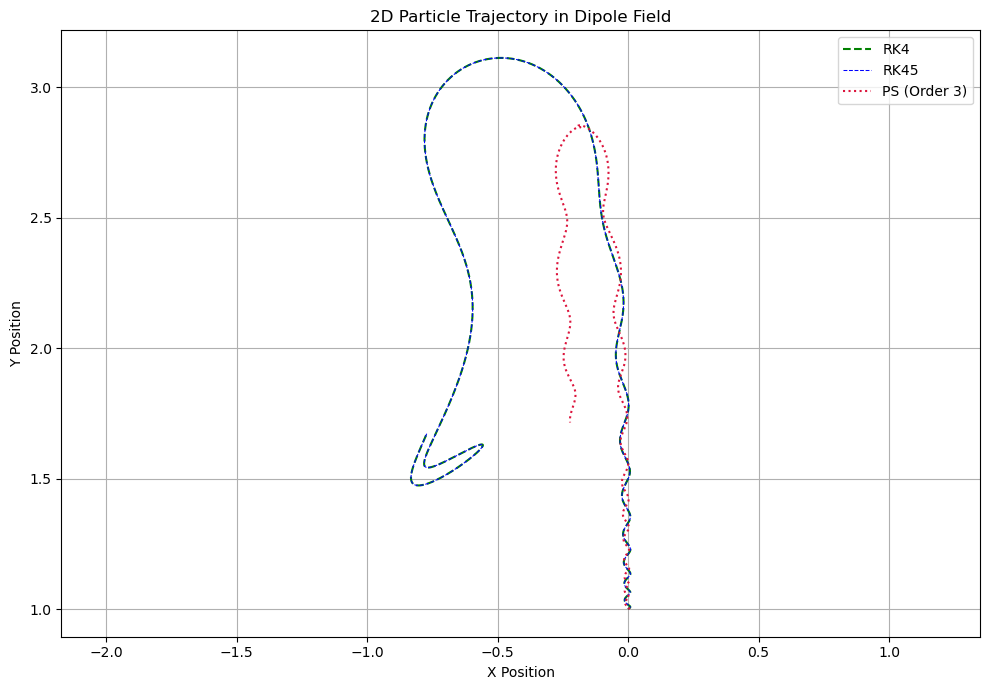
\includegraphics[width=\textwidth]{Images/Dipole/Dipole_slow_PS_Order3_traj_qm2_400s.png}
%             \caption{2D particle trajectories in a dipole field showing divergence of RK methods from PS model for a low-velocity charged particle.}
%             \label{FIG:Dipole_traj_400s}
%         \end{minipage}%
%         \hfill
%         \begin{minipage}[t]{0.45\textwidth}
%             \centering
%             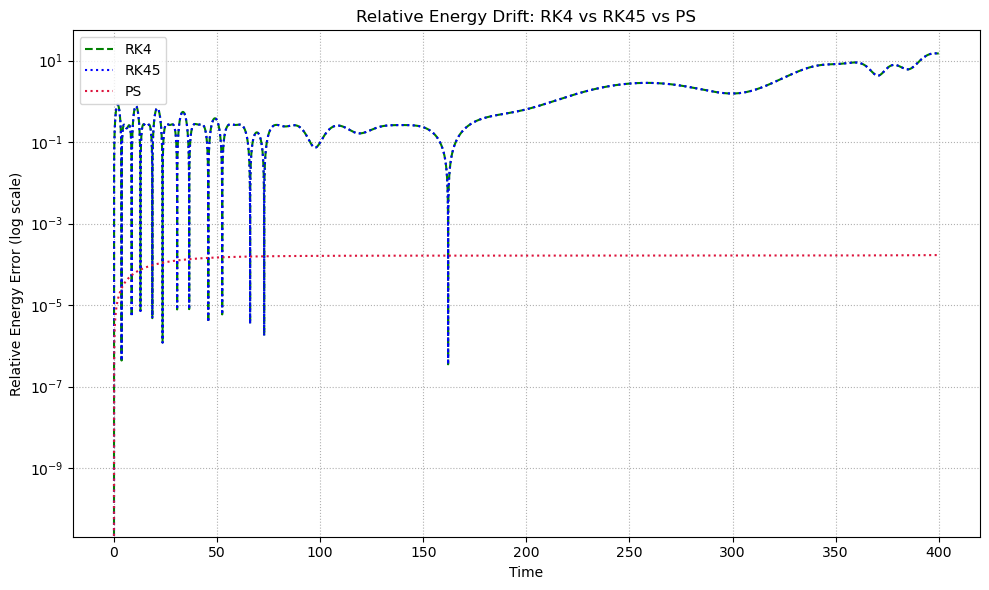
\includegraphics[width=\textwidth]{Images/Dipole/Dipole_slow_PS_Order3_error_qm2_400s.png}
%             \caption{Energy drift of a low-velocity charged particle in a dipole field computed using the Parker–Sochacki method and two different Runge-Kutta methods (fixed-step fourth order, RK4, and adaptive, RK45).}
%             \label{FIG:Dipole_error_400s}
%         \end{minipage}
%     \end{figure}
The PS method was able to maintain stable simulation of the particle trajectory in a dipole field and continued to exhibit the characteristic bounce 
 and drift motion, Figure \ref{FIG:Dipole_drift} and Figure \ref{FIG:Dipole_bounce}, for an extended period of time, 5000 units in scaled time.
    \begin{figure}[H]
        \centering
        \begin{minipage}[t]{0.4\textwidth}
            \centering
            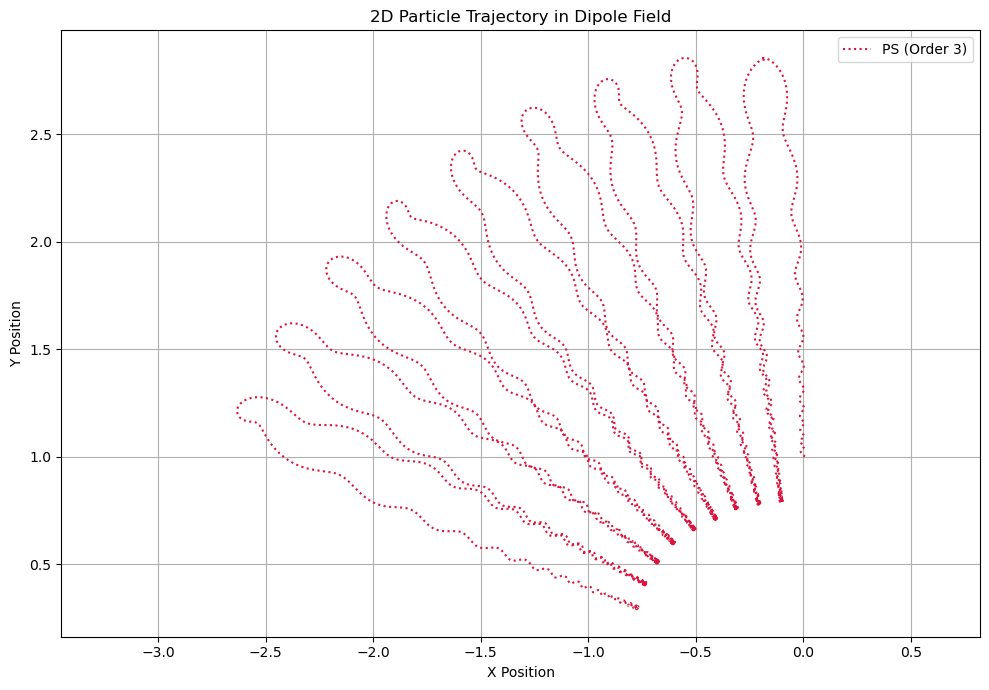
\includegraphics[width=\textwidth]{Images/Dipole/Dipole_slow_PS_Order3_traj_qm2_5000s.png}
            \caption{Low-velocity charged particle in a magnetic dipole exhibiting characteristic bounce and drift in x-y plane using PS method.}
            \label{FIG:Dipole_drift}
        \end{minipage}%
        \hfill
        \begin{minipage}[t]{0.45\textwidth}
            \centering
            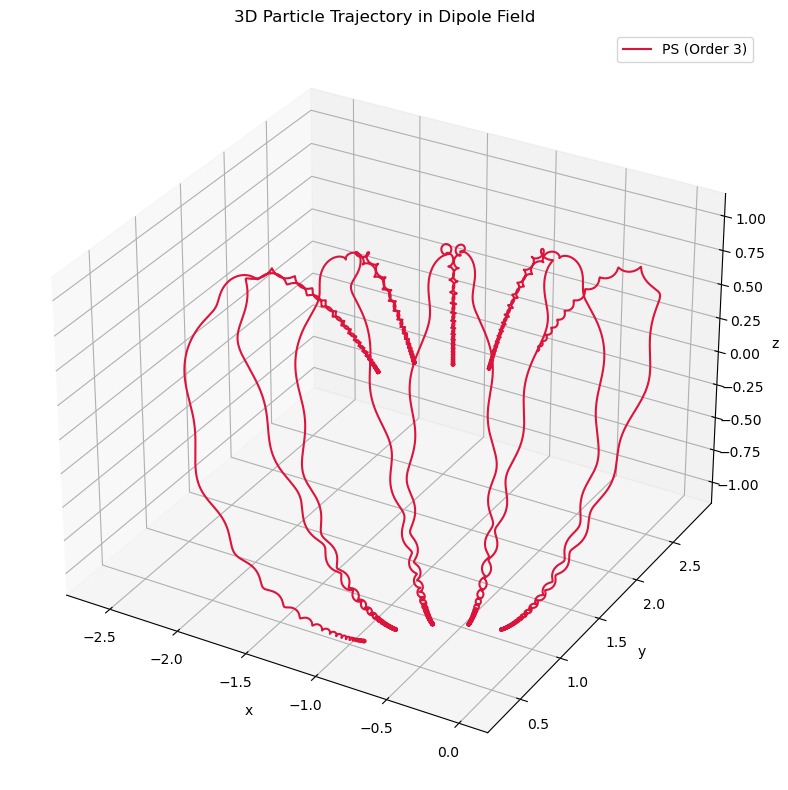
\includegraphics[width=\textwidth]{Images/Dipole/Dipole_slow_PS_Order3_3Dtraj_qm2_5000s.png}
            \caption{Low-velocity charged particle in a magnetic dipole exhibiting characteristic bounce and drift in 3-D using PS method.}
            \label{FIG:Dipole_bounce}
        \end{minipage}
    \end{figure}



While a comprehensive parameter sweep was beyond the scope of this study, initial analysis indicates that the PS method presents a viable solution for simulating particle motion in dipole fields and under conditions where traditional methods struggle with stability and energy conservation, it may work as an alternative with a careful selection of parameters.\\


\section{Concluding Observations}
This paper has investigated the Parker-Sochacki (PS) method as a viable approach for simulating charged particle motion in magnetic fields, providing a detailed comparison with the established Runge-Kutta techniques (RK4 and RK45). The results demonstrate that the PS method, when properly formulated, is capable of producing accurate and stable trajectories across a range of magnetic field configurations, including constant, hyperbolic, and dipole fields. While Runge-Kutta methods remain a powerful and widely used tool, the PS method offers a distinct alternative, grounded in power series expansions and auxiliary variables. It is important to acknowledge that the PS method often involves an upfront cost in terms of the analytical effort required to derive the power series equations and auxiliary variable relationships specific to each problem. Furthermore, while the PS method often required a smaller time step compared to Runge-Kutta methods, its computational cost per step can be lower due to its reliance on simple algebraic operations. However, reducing the time step excessively should be handled with care, as the power series expansions are proportional to $t^n$, where $n$ is the PS order, can lead to early truncation errors if the time step is too small, effectively limiting the accuracy of the approximation.\\

It's important to address that this study did not focus on maximizing code efficiency for any of the methods, nor did it conduct a full parameter sweep to comprehensively evaluate their performance across all possible scenarios. This purpose of this study was to highlight the PS method as a functional and potentially valuable tool for simulating charged particle dynamics, expanding the available options for researchers and providing a basis for further exploration and optimization. Future work could focus on adaptive step-size control for the PS method and investigation of its performance in more complex, realistic magnetic field environments, as well as code optimization to improve computational efficiency. The intent of this paper is not to promote one method over another, but rather to demonstrate the practical viability of the PS method.


\pagebreak
\printbibliography

\end{document}





